\documentclass[dvipdfmx,9pt,notheorems]{beamer}
%%%% 和文用 %%%%%
\usepackage{bxdpx-beamer}
\usepackage{pxjahyper}
\usepackage[absolute,overlay]{textpos}
\usepackage{minijs}%和文用
\renewcommand{\kanjifamilydefault}{\gtdefault}%和文用

%%%% スライドの見た目 %%%%%
\usetheme{metropolis}
\usefonttheme{professionalfonts}
\usecolortheme[RGB={112,128,144}]{structure}
\setbeamertemplate{frametitle}[default][center]
\setbeamertemplate{navigation symbols}{}
\setbeamercovered{transparent}%好みに応じてどうぞ)
\setbeamertemplate{footline}[page number]
\setbeamerfont{footline}{size=\normalsize,series=\bfseries}
\setbeamercolor{footline}{fg=black,bg=black}
%%%%

%%%% 定義環境 %%%%%
\usepackage{amsmath,amssymb}
\usepackage{amsthm}
\theoremstyle{definition}
\newtheorem{theorem}{定理}
\newtheorem{definition}{定義}
\newtheorem{proposition}{命題}
\newtheorem{lemma}{補題}
\newtheorem{corollary}{系}
\newtheorem{conjecture}{予想}
\newtheorem*{remark}{Remark}
\renewcommand{\proofname}{}
%%%%%%%%%

%%%%% フォント基本設定 %%%%%
\usepackage[T1]{fontenc}%8bit フォント
\usepackage{textcomp}%欧文フォントの追加
\usepackage[utf8]{inputenc}%文字コードをUTF-8
\usepackage{otf}%otfパッケージ
\usepackage{sansmathfonts}%数式・英文ローマン体を sansmathfonts にする
\usepackage{bm}%数式太字
%%%%%%%%%%

\title{FreeFlow: Software-based Virtual RDMA Networking for Containerized Clouds}
\author{Daehyeok Kim\footnotemark[1], Tianlong Yu\footnotemark[1], Hongqiang Harry Liu\footnotemark[3], Yibo Zhu\footnotemark[2], Jitu Padhye\footnotemark[2], Shachar Raindel\footnotemark[2], Chuanxiong Guo\footnotemark[4], Vyas Sekar\footnotemark[1], Srinivasan Seshan\footnotemark[1]}
\institute{\footnotemark[1]Carnegie Mellon University, \footnotemark[2]Microsoft, \footnotemark[3]Alibaba, \footnotemark[4]Bytedance}

\begin{document}

\begin{frame}[plain]\frametitle{}
\titlepage %表紙
\end{frame}

\begin{frame}\frametitle{Contents}
\raggedright
\tableofcontents
\end{frame}

\section{概要}
\begin{frame}\frametitle{概要}
\begin{itemize}
  \item コンテナを利用した大規模クラウドアプリケーション
  	\begin{itemize}
  		\item high resource efficiency
  		\item	light weight isolation
  	\end{itemize}
	\item その一方でdata-intensiveなアプリケーション(deeplearning, data analytics)は高性能のネットワーク(RDMA)を要求する
	\item コンテナ化によるメリットとRDMAによるメリットをいいとこ取りしたい! $\rightarrow$ \bm{{\color{red} FreeFlow}}
\end{itemize}
\end{frame}
\section{目的・背景}
\begin{frame}\frametitle{背景}
\begin{itemize}
  \item コンテナ化のコアメリットは効率的で柔軟なアプリケーションマネジメントの提供である。
	\item containerized cloudではネットワークについて以下の要件をコンテナが満たしていてほしい
	\begin{itemize}
		\item \textit{{\color{red} Isolation}} : containerはそれぞれのnamespaceを持っていてほしい
		\item \textit{{\color{red} Portability}} : virtual network (overlay network) を利用してコンテナ間通信できてほしい
		\item \textit{{\color{red} Controllability}} : control / data plane policy をコントロールできてほしい
	\end{itemize}
  \item RDMAの完全仮想化は性能を殺してしまうし、RDMA自体はcontrol / data plane のpolicy変更が難しい(HWに寄るため)
	\begin{itemize}
		\item 実際のところ、TensorFlowやSparkなどは専用ベアメタル + RDMAなどの形態で運用しパフォーマンスを担保するケースがある。
		\item これは提供側にとってもユーザ側にとっても辛い
	\end{itemize}
\end{itemize}
\end{frame}

\begin{frame}\frametitle{目的}
	\begin{itemize}
		\item \bm{目的} : container環境でもRDMAが使えて、ベアメタル + RDMAくらいの性能が出るようにする!
		\item \textit{Isolation}, \textit{Portability}, \textit{Controllability} に加えて、\textit{high performance} も達成する!
		\item containerから利用できるRDMAのその他の手法に関してまとめたものが下図
	\end{itemize}
  \begin{figure}[htb]
    \centering
    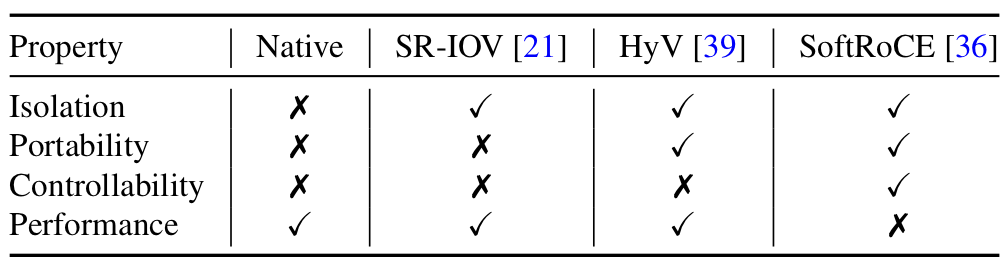
\includegraphics[scale=1]{fig/table1.png}
  \end{figure}%
\end{frame}
\section{FreeFlow}
\begin{frame}\frametitle{FreeFlowの概要}
	\begin{itemize}
		% TODO: shadow memoryの話は詰めたい
		\item RDMAではAPIを利用してアプリケーションが直接HW NICにコマンドを投げる
		\item FreeFlowではこのアプリケーションとHW NICの間に割って入る。
		\begin{itemize}
			\item FreeFlow Router (以降, FFR) は同一ホストの別コンテナとして起動しておく。
			\item FFRでvirtual networkの提供 + control / data plane policyの適用。
			\item FFRは各contianerのmemory領域をshareしていて、App $\rightarrow$ NIC も NIC $\rightarrow$ App もここのメモリを橋渡しにする。
			\item 同じ物理メモリを利用している(これがshadow memory?)ためzero-copy (FFR $\rightarrow$ App)
		\end{itemize}
	\end{itemize}
	% figure2-a, figure2-bを入れる
\end{frame}

% vebsの話はどうしようね...

\begin{frame}\frametitle{Architecture}
	% ここはなんとか説明したい
	\begin{itemize}
		\item グレーの部分がFreeFlowで修正した部分
  \end{itemize}
  \begin{figure}[htb]
    \centering
    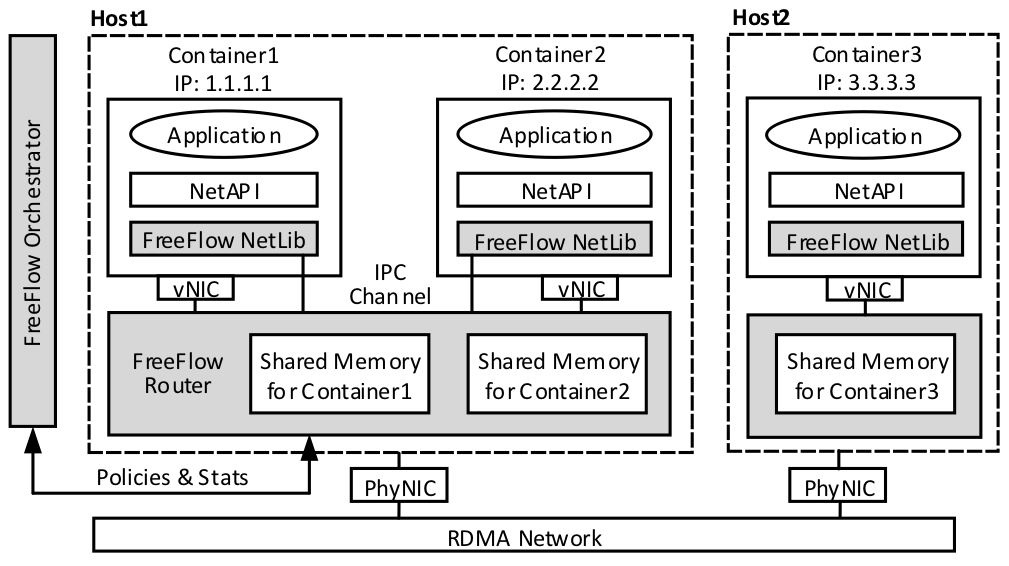
\includegraphics[scale=1]{fig/figure4.png}
  \end{figure}
\end{frame}

\begin{frame}\frametitle{FreeFlow Library (FFL)}
	\begin{itemize}
		\item Appコンテナ内部でAppに \\
			    FreeFlow transparentを提供する
		\item ただし、{\color{orange} App内部からは通常のRDMA \\
			    Verbs library を利用しているようにしか見えない}
		\item Appはコードの修正なし \\
			    (もしくはほんの少しの修正)に利用できる
		\item FFRとやり取りする
  \end{itemize}
  \begin{textblock*}{0.4\linewidth} (230pt, 100pt)
  	\centering
		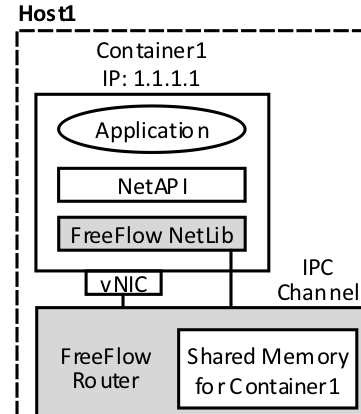
\includegraphics[width=30mm]{fig/figure4-ffl.png}
  \end{textblock*}
\end{frame}

\begin{frame}\frametitle{FreeFlow Router (FFR)}
	\begin{itemize}
		\item 各ホストでシングルインスタンス(コンテナ)として起動し、そのホストの各コンテナにvirtual networkの提供を行う
		\item FFLとのchannelをコントロールすることで、data planeのリソースポリシー(QoSなど)を実装する
		\item message-level eventのハンドリングになる。
		\item FFOと連携し、IPアドレスなどのタスク処理も行う
  \end{itemize}
  \begin{figure}[htb]
    \centering
    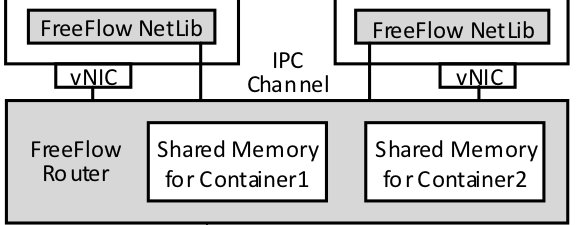
\includegraphics[scale=1]{fig/figure4-ffr.png}
  \end{figure}
\end{frame}

\begin{frame}\frametitle{FreeFlow Orchestrator (FFO)}
	\begin{itemize}
		\item コントロールプレーンを司る \\
			   (らしいが論文を通してあまり説明が無い。。。)
		\item コンテナ通信のコントロールや \\
			    クラスタのリアルタイムモニタリングなど。
		\item メモリマップの保持もここで行っている
  \end{itemize}
  \begin{textblock*}{0.4\linewidth} (230pt, 100pt)
  	\centering
  	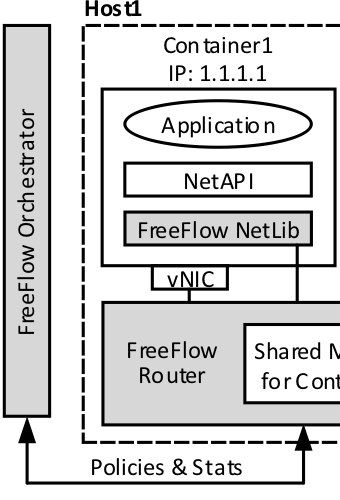
\includegraphics[width=30mm]{fig/figure4-ffo.png}
  \end{textblock*}
\end{frame}

\section{Transparent Support for RDMA operation}
% まず大きな概要だけ書いて(後の理解に必要)詳細は再度考える
\begin{frame}\frametitle{Transparent Support for RDMA operation}
	\begin{itemize}
		\item これどこまでかこうかね...
	\end{itemize}
\end{frame}

% ここの話は性能に関わるのでいる
% RPCの話はまぁしなくていいだろう
\section{Communication channel between FFL and FFR}
\begin{frame}\frametitle{Communication Channel between FFL and FFR}
	\begin{itemize}
		\item FFLとFFRの間のCommunication Channelについて。
		\item FFR側ではAppがRDMAに対して行ったリクエスト(APIコール)を模倣する必要がある。
		\item 2つの考え方がある。
		\begin{itemize}
			\item Unix file descriptorを利用する
			\item Fastpathを利用する
		\end{itemize}
	\end{itemize}
\end{frame}

% Queuenの話が出てきちゃった。。。
\begin{frame}\frametitle{Verbs forwarding via File Descriptor}
	\begin{itemize}
		\item APIコール自体をRPCのように模倣するのではなく、NIC fdに対して行われる要求をFFR側で模倣する。
		\item コンテナ内部のNIC fdをUnix domain socketに差し替える。もう片方の終端はFFR。
		\item FFRはコンテナ内の仮想Queueへの操作を物理NICの実際のQueueへの同じ操作にmappingする。逆の通信も同様の動きをする。
		% TODO: ここはもう少し詳細に語れるようになりたいな。
		% \item 物理NICからの応答も、仮想Queueを持つ仮想NICからの応答に変換し、Unixソケットを通じてFFLに応答を返す。
	\end{itemize}
  \begin{figure}[htb]
    \centering
    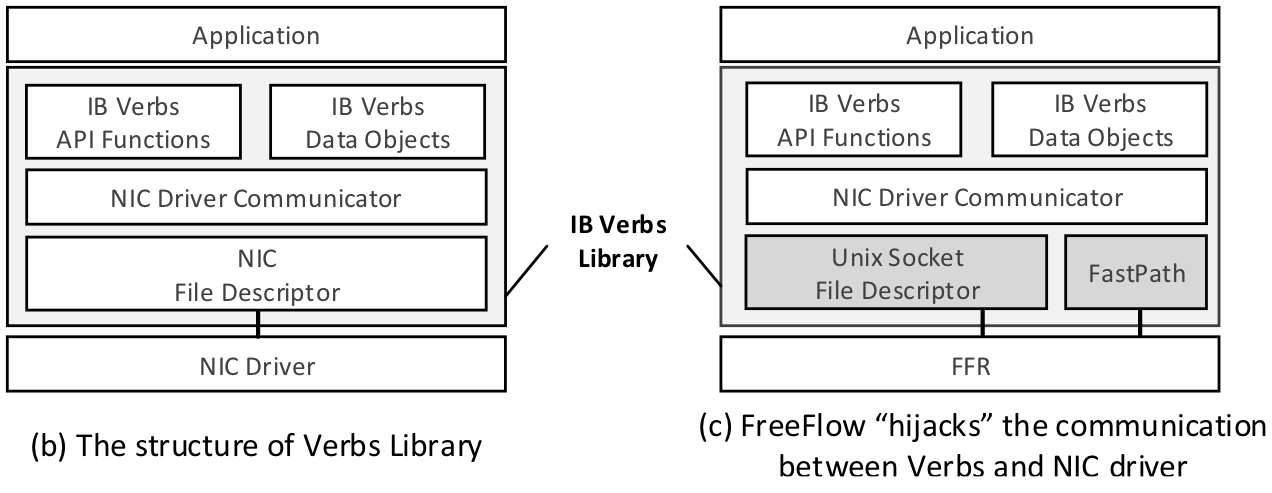
\includegraphics[scale=1]{fig/figure7-bc.png}
  \end{figure}
\end{frame}

\begin{frame}\frametitle{File Discriptor方式の欠点}
	\begin{itemize}
		\item レイテンシが大きい。ラウンドトリップタイムを計測したらかんたんに$5\mu$sを超える。
		\item レイテンシセンシティブなアプリケーションでは致命的。。。
		\item ただし、CPUはほとんど使わない $\rightarrow$ ボトルネックの解消にCPUリソースを少しだけ拝借する設計 \bm{{\color{red} Fastpath}} を考えた
	\end{itemize}
\end{frame}

\begin{frame}\frametitle{Fastpath between FFL and FFR}
	\begin{itemize}
		\item FFLとFFRでメモリを共有する方式。
		\begin{enumerate}
			\item まずFFRがCPUを回し、FFLからのリクエスト、すなわちメモリなにか書かれないか確認する。
			\item リクエストを受け取ったらFFRは直ちに処理する、その際FFLもCPUを回しレスポンスを確認する。
			\item レスポンスが帰ってきたら直ちに処理し、FFL側はCPUを手放す。
	  \end{enumerate}
	\end{itemize}
  \begin{figure}[htb]
    \centering
    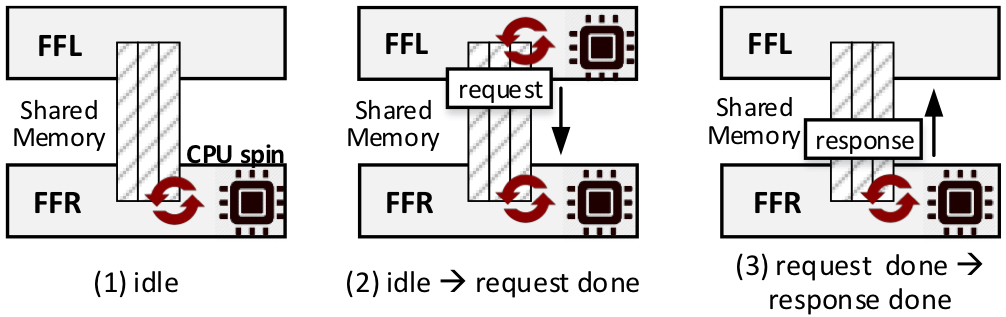
\includegraphics[scale=1]{fig/figure8.png}
  \end{figure}
\end{frame}

\begin{frame}\frametitle{Fastpath方式の欠点と対策のための実装}
	\begin{itemize}
		\item CPU overheadがある。
		\begin{itemize}
			\item 1FFR(つまり1ホスト)で1CPUのみ利用する。複数コンテナの着信確認は1CPUで行うようにデザインした。
			\item データパス上にあり、且つnon-blockingな関数のときにのみ利用される(?)ため、FFL側でのCPU利用時間は極めて小さい。
		\end{itemize}
		\item FFOはホスト上にレイテンシセンシティブなアプリケーションが無いことを知っている場合(これはコンテナイメージの実行で判断?)、FastpathとCPUの利用を止めることができる。
	\end{itemize}
\end{frame}

\section{Discussion}
\begin{frame}\frametitle{CPU overhead}
	\begin{itemize}
		\item 今回はperformanceためにあえて許容した。
		\item CPUがやるべき仕事をhardwareにオフロードできれば解決は可能かもね。
		\item future workの一つ
	\end{itemize}
\end{frame}

\begin{frame}\frametitle{Security}
	\begin{itemize}
		\item FFRで各コンテナのメモリ状態を取りまとめているから、同一ホストだしIPC領域スキャンすれば確認できるのでは?
		\begin{itemize}
			\item FFRは個々のQPに共有メモリバッファを作成する、つまりコンテナ内部に存在する共有メモリが、コンテナの仮想メモリアドレスにマッピングされるため問題ない。
		\end{itemize}
		\item memory key(?)の問題. これはFreeFlowというよりraw RDMAにおけるone-sided operationの問題であり、FreeFlowで別段悪化するなどはない。
	\end{itemize}
\end{frame}

\begin{frame}\frametitle{Work with external legacy peer}
	\begin{itemize}
		\item FFRはリモートのpeerがFFR使ってるか普通のRDMAかなどの判別をするわけではないため、RDMAで普通に通信可能。
	\end{itemize}
\end{frame}

\begin{frame}\frametitle{Container migration}
	\begin{itemize}
		\item offline migration(shutdown $\rightarrow$ move $\rightarrow$ reboot)可能。
		\item IPアドレスは変わらないので、rebootしたらRDMA connectionを再確立させることができる。
		\item live migrationはできない。
	\end{itemize}
\end{frame}

\begin{frame}\frametitle{VM host}
	\begin{itemize}
		\item 今回のprototypeでは基本的にベアメタル上にコンテナを起動させているが、physical NICにアクセスできればいいので、SR-IOVなどを利用しているVM上なら可能。
	\end{itemize}
\end{frame}

\begin{frame}\frametitle{Congestion control}
	\begin{itemize}
		\item RDMA NICに輻輳制御メカニズムは入っており、FreeFlowはそれに準拠する。
	\end{itemize}
\end{frame}

% Discussionの内容は適宜入れるかまとめる
\section{評価}
\begin{frame}\frametitle{構成}
	\begin{enumerate}
		\item Infiniband
		\begin{itemize}
			\item CPU : Intel Xeon E5-2620 2.10GHz 8-core $\times$ 2
			\item RAM : 64GB
			\item NIC : 56Gbps Mellanox FDR CX3
			\item OS  : Ubuntu 14.04 (3.13.0-129-generic)
		\end{itemize}
		\item RoCE
		\begin{itemize}
			\item CPU : Intel Xeon E5-2609 2.40GHz 4-core
			\item RAM : 64GB
			\item NIC : 40Gbps Mellanox CX3 NIC
			\item OS  : Ubuntu 14.04 (4.4.0-31-generic)
		\end{itemize}
		\item その他
		\begin{itemize}
			\item Container Runtime : Docker (v1.13.0)
			\item Virtual Network   : Weave (v1.8.0)
			\item OvS kernel module : enabled
		\end{itemize}
	\end{enumerate}
\end{frame}

\begin{frame}\frametitle{Microbenchmark: Throughput and Latency}
	\begin{itemize}
		\item ib\_send\_lat, ib\_send\_bw でtwo-sided operation (SEND) のlatency, bandwidthの測定
		\item ib\_write\_lat, ib\_write\_bw でone-sided operation (WRITE) のlatency, bandwidthの測定
		\item これらのツールはFreeFlow上で{\color{orange}コードの変更なしに実行できた}
		\item inter-hostとintra-hostを区別しないため(?)、inter-host performance valueを計測した。(なんかあとでLatency計測のときにThroughputと同じようにとか言いながらToR越しに接続しているのでなんともわからん。/あーinterhost文しか計測してないぞという話か?)
	\end{itemize}
\end{frame}

\begin{frame}\frametitle{Microbenchmark: Throughput}
	\begin{itemize}
		\item 2種類のtestbedでRDMA SEND/WRITEのスループットを測定。
		\item 1GBのデータを2KB〜1MBの単位で分割して転送している。
		\item Host-RDMAはベアメタル + RDMAの性能
		\item message size $\geq$ 8KBの場合、Infiniband/RoCEともにベアメタルの性能と同じになる。
		\item (WRITEのデータはREADよりわずかに良いらしいが論文からは省略されている。)
	\end{itemize}
  \begin{figure}[htb]
    \centering
    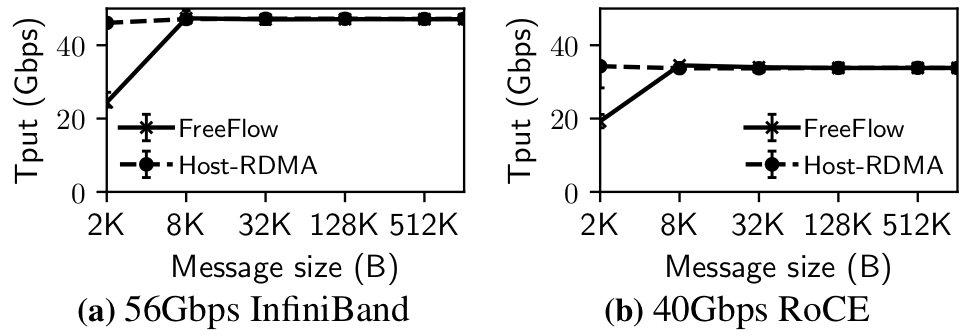
\includegraphics[scale=1]{fig/figure9.png}
  \end{figure}
\end{frame}


\begin{frame}\frametitle{Microbenchmark: Throughput}
	\begin{itemize}
			\item message size $\leq$ 8KBの場合について、同時稼働コンテナ数(flow数)を512にスケールアップしたところブラフがベアメタル + RDMAとほぼ同じになった。
			\item このときの帯域幅は各フローで均等に分散していることも Jain's fairness index により確認した。
			\item 細かすぎてlatencyに食われる分、Throughputが飽和していなかっただけのよう。(実際2CPUをFRRに利用する方法でもうまく行ったらしい)
	\end{itemize}
  \begin{figure}[htb]
    \centering
		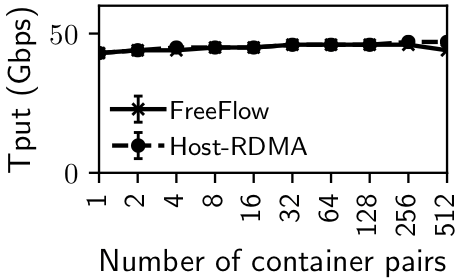
\includegraphics[scale=1]{fig/figure11.png}
  \end{figure}
\end{frame}

\begin{frame}\frametitle{Microbenchmark: Latency}
	\begin{itemize}
		\item 64B, 256B, 1KB, 4KBのメッセージを送信し、レイテンシを測定した。
		\item one-sidedであるWRITEのほうが、two-sidedであるSENDよりレイテンシが少なく、FreeFlowとベアメタルの間のギャップも小さい。
		\item とはいえSENDの場合であっても余剰Latencyは1.5$\mu$s程度。
		\item これはFFLとFFRの間のIPCによるレイテンシで、WRITEの場合はtriggerが1回だけど、SENDの場合は2回なのが効いているから。
	\end{itemize}
  \begin{figure}[htb]
    \centering
		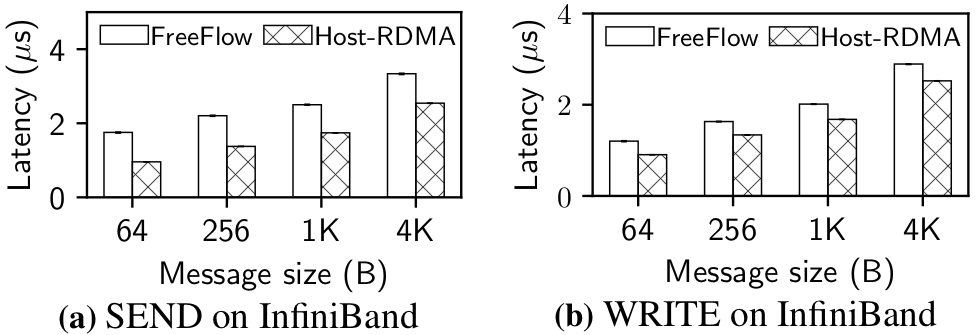
\includegraphics[scale=1]{fig/figure10.png}
  \end{figure}
\end{frame}

\begin{frame}\frametitle{Microbenchmark: Latency}
	\begin{itemize}
		\item ちなみに、1.5$mu$sってどんれくらい?
		\item ネットワークのone hop : 0.55$mu$s
		\item TCP stack : least 10$mu$s
		\item TCP virtual network latency : 40$mu$s以上(彼らのテストでは)
		\item $\rightarrow$ {\color{red}FreeFlowはcontainer virtual networkを有効にした状態でRDMAのlatency advantageを保存できている!}
	\end{itemize}
\end{frame}

\begin{frame}\frametitle{Microbenchmark: CPU overhead}
	\begin{itemize}
		\item Fastpath enableの場合とそうでない場合は実際どのくらいレイテンシに差が出るか。
		\begin{itemize}
			\item Fastpathだと2.4$\mu$sだが、disableすると17.0$\mu$sまで上昇する。
		\end{itemize}
	\item Throughput測定時(このときどのパターンでも帯域はフルに使っており、message sizeは1MB)のCPU UtilizationはやはりLowCPU(disable Fastpath)のほうが断然良い。
	\item {\color{orange}ワークロードによって使い分けるのがベスト}
  \end{itemize}
  \begin{figure}[htb]
  	\centering
		\begin{tabular}{c}
			\begin{minipage}{0.4\hsize}
  			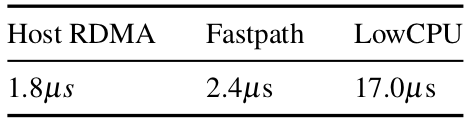
\includegraphics[scale=1]{fig/table3.png}
  		\end{minipage}
			\begin{minipage}{0.4\hsize}
  			\centering
  			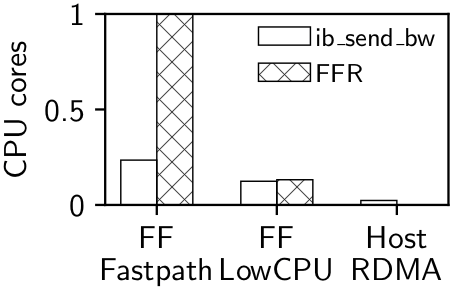
\includegraphics[scale=1]{fig/figure12.png}
  		\end{minipage}
		\end{tabular}
  \end{figure}
\end{frame}

% 6章のrate limiterの話を書いてない。。。。
\begin{frame}\frametitle{Microbenchmark: Rate limiter and Performance Isolation}
	\begin{itemize}
		\item rate limiterの性能を検証した
		\item Infinibandのtestbedで、異なるホストのコンテナ間で単一のフローを開始した。
		\item flow rateに制限をかけ、帯域幅を1Gbps〜40GBpsまで変更して測定した。
		\item 図から分かる通り理想通りにリミットがかかっている。これを6のCPU overheadで実現している。
		\item これはコンテナペア間で分離できており、それぞれに制限をかけても問題なく動いた。
	\end{itemize}
  \begin{figure}[htb]
    \centering
		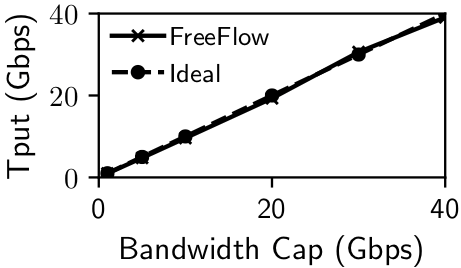
\includegraphics[scale=1]{fig/figure13.png}
  \end{figure}
\end{frame}

% 個々らへん理由とかはちゃんと言えるようにする。(書いてある。m)
\begin{frame}\frametitle{Microbenchmark: TCP socket over RDMA}
	\begin{itemize}
		\item 本説とは少しずれる気がするが、socket-based applicationについても利益をもたらすよという話。
		\item 通常のTCP/IP virtual networkに比べて、rsocketを利用してFreeFlowでRDMAすると早い。
		\item iperfでTCP throughputを、NPtcpを利用してTCP latencyをそれぞれ計測した。({\color{orange}これらも変更の必要はなかった})
		\item Weaveと比べると常に早く、Throughputでホストに勝てないのはsocketとverbsの変換部分のoverhead。
	\end{itemize}
  \begin{figure}[htb]
    \centering
		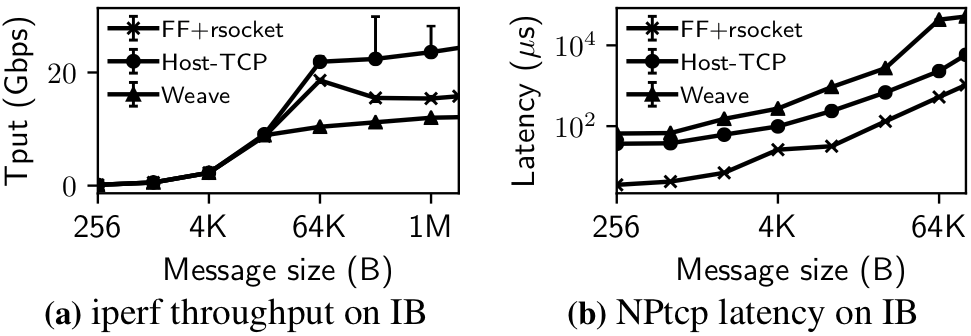
\includegraphics[scale=1]{fig/figure14.png}
  \end{figure}
\end{frame}


\begin{frame}\frametitle{Real-world application}
	\begin{itemize}
		\item TensorflowとSparkを利用して機械学習とデータアナリティクスの性能を確認した。
		\item 比較対象はHost-RDMA(これに近づくほど理想的)、Host-TCP, Weaveの三種類。
		\item これらはすべてInfiniband構成で実行した。
	\end{itemize}
\end{frame}

\begin{frame}\frametitle{Tensorflow}
	\begin{itemize}
		\item 3台のサーバ上でRDMA対応のTensorflowを実行。({\color{orange}変更は一行})
		\item 各サーバにはNVIDIA GTX 1080Ti $\times$ 3がそれぞれ搭載されており、一基がmasterかつparameterサーバ, それ以外がworkor
		\item 2種類のtraining workloadを実行する
		\begin{itemize}
			\item Convolutional Neural Network : 画像認識用途
			\item Recurrent Neural Network : 音声認識用途
		\end{itemize}
	\end{itemize}
\end{frame}

\begin{frame}\frametitle{Tensorflow: CNN}
	\begin{itemize}
		\item 3種類のモデル(ResNet-50, Inception-v3, AlexNet)をtraining dataとしてsynthetic ImageNet dataを利用。
		\item 分散トレーニングにおいてネットワークパフォーマンスがボトルネックになる。
		\begin{enumerate}
			\item Host-RDMAとHost-TCPの比較をするとRDMAのほうが1.8〜3倍程度良い。
			\item FreeFlowとWeaveを比較するとより大きい差がでている。(Alexnetに関しては14.6倍ほどRDMAのほうが良い)
		\end{enumerate}
		\item FreeFlowの性能はHost-RDMAに切迫している!(Alexnetは少し高いがこれはノイズだろうとのこと)
	\end{itemize}
  \begin{figure}[htb]
    \centering
		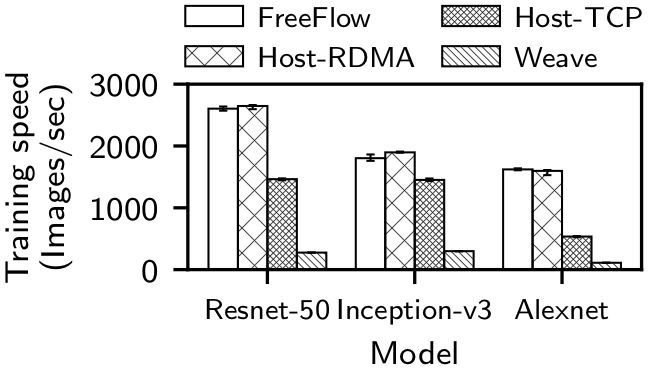
\includegraphics[scale=1]{fig/figure15-a.png}
  \end{figure}
\end{frame}

\begin{frame}\frametitle{Tensorflow: RNN}
	\begin{itemize}
		\item エンコーダ/デコーダとか隠れ層とかの設定の話があったがちょっと良くわからなかった。。。
		\item 各訓練ステップに費やされた時間をCDFにしたグラフ
		\item CNNの場合と同様に、FreeFlowはHost-RDMAに切迫しており、Weaveに比べて8.7倍くらいの性能が出ている
	\end{itemize}
  \begin{figure}[htb]
    \centering
		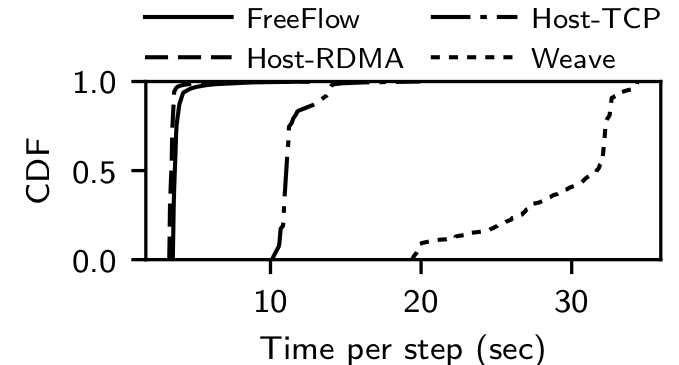
\includegraphics[scale=1]{fig/figure15-b.png}
  \end{figure}
\end{frame}

\begin{frame}\frametitle{Spark}
	\begin{itemize}
		\item 2つのサーバーでSparkを実行。片方にはmaster, slaveのcontainer, もう片方にはslave containerで動作。
		\item Sparkに同梱されている、\textit{GroupBy}と\textit{SortBy}のベンチマークで計測した。
		\item 結果的に、Tensorflowと同様の結果になり、ネットワーク性能がアプリケーション性能に大きく影響しているのがわかる。
		\item FreeFlowはHost-RDMAに切迫しており、Weaveに比べて1.8倍の性能がでる。
	\end{itemize}
  \begin{figure}[htb]
    \centering
		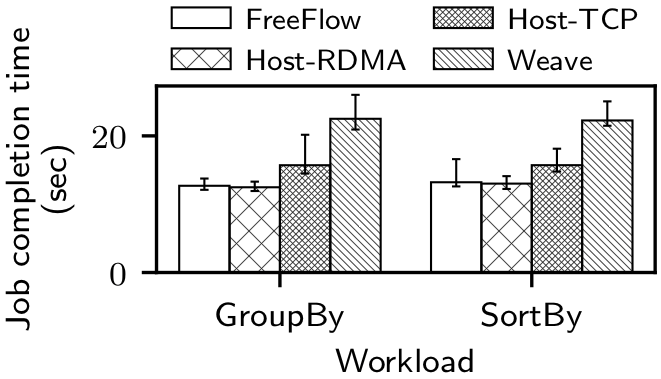
\includegraphics[scale=1]{fig/figure16.png}
  \end{figure}
\end{frame}

\section{結論}
\begin{frame}\frametitle{結論}
	\begin{itemize}
    \item FreeFlowにより、コンテナ環境に対して、\textit{Isolation}、\textit{Portability}、\textit{Controllability}、\textit{Performance}を満たすRDMA環境を提供することができた。
  	\item 肝心のPerformanceに関してもベアメタルRDMAに匹敵するくらいの性能が出る。
		\item Githubは\href{https://github.com/microsoft/Freeflow}{こちら}
	\end{itemize}
\end{frame}

\newcounter{finalframe}
\setcounter{finalframe}{\value{framenumber}}
\setcounter{framenumber}{\value{finalframe}}
\end{document}
